\documentclass[paperwidth=48in,paperheight=48in, fontscale=0.4166666666666, landscape]{baposter}

\usepackage[T1]{fontenc}
\usepackage[utf8]{inputenc}

\usepackage{amsfonts, amsmath, amssymb}
\usepackage{mathtools}

\usepackage{pifont}


\usepackage{graphicx}
\usepackage{subfig}
\usepackage{epsfig}
\usepackage{color}

\graphicspath{{/hdd/Documents/math-cnn-derivation-swedish-paper/English/images}}

\usepackage{url}
%%  Defines the command \url{} that can be used to typeset url:s
%%  in text

\usepackage[parfill]{parskip}
\usepackage{ragged2e}

\setcounter{tocdepth}{4}
\setcounter{secnumdepth}{4}


\newcommand*{\pd}[2]{\ensuremath{\dfrac{\partial #1}{\partial #2}}}
\newcommand*{\inpd}[2]{\ensuremath{\frac{\partial #1}{\partial #2}}}
\DeclarePairedDelimiter\floor{\lfloor}{\rfloor}

\usepackage{wrapfig}
\usepackage{lmodern}

\usepackage[utf8]{inputenc} %unicode support
\usepackage[T1]{fontenc}


\selectcolormodel{cmyk}

\graphicspath{{figures/}} % Directory in which figures are stored


\newcommand{\compresslist}{%
\setlength{\itemsep}{0pt}%
\setlength{\parskip}{1pt}%
\setlength{\parsep}{0pt}%
}

\newenvironment{boenumerate}
  {\begin{enumerate}\renewcommand\labelenumi{\textbf\theenumi.}}
  {\end{enumerate}}



\begin{document}


\definecolor{darkgreen}{cmyk}{0.8,0,0.8,0.45}
\definecolor{lightgreen}{cmyk}{0.8,0,0.8,0.25}

\begin{poster}
{
grid=false,
headerborder=open, % Adds a border around the header of content boxes
colspacing=2.5em, % Column spacing
bgColorOne=white, % Background color for the gradient on the left side of the poster
bgColorTwo=white, % Background color for the gradient on the right side of the poster
borderColor=darkgreen, % Border color
headerColorOne=lightgreen, % Background color for the header in the content boxes (left side)
headerColorTwo=lightgreen, % Background color for the header in the content boxes (right side)
headerFontColor=white, % Text color for the header text in the content boxes
boxColorOne=white, % Background color of the content boxes
textborder=rounded, %rectangle, % Format of the border around content boxes, can be: none, bars, coils, triangles, rectangle, rounded, roundedsmall, roundedright or faded
eyecatcher=false, % Set to false for ignoring the left logo in the title and move the title left
headerheight=0.0\textheight, % Height of the header
headershape=rounded, % Specify the rounded corner in the content box headers, can be: rectangle, small-rounded, roundedright, roundedleft or rounded
headershade=plain,
headerfont=\Large\textsf, % Large, bold and sans serif font in the headers of content boxes
%textfont={\setlength{\parindent}{1.5em}}, % Uncomment for paragraph indentation
linewidth=4pt % Width of the border lines around content boxes
}
{}
%
%----------------------------------------------------------------------------------------
%	TITLE AND AUTHOR NAME
%----------------------------------------------------------------------------------------
%
{
\textsf %Sans Serif
{%TITLE HERE
}
} % Poster title
% {\vspace{1em} Marta Stepniewska, Pawel Siedlecki\\ % Author names
% {\small \vspace{0.7em} Department of Bioinformatics, Institute of Biochemistry and Biophysics, PAS, Warsaw, Pawinskiego 5a}} % Author email addresses
{%more info
}
{} % University/lab logo


\headerbox{Introduction}{name=introduction,column=0,row=0, span=1}{
The project is split into the following three parts: (1) the derivation of the general case for a convolutional neural network (CNN) with an arbitrary input of a tensor of order 4 for usage in our own neural network library implementation, (2) the systematic construction and evaluation of a fully convolutional model for detecting a variable number of faces for real time video, and (3) the improvement of temporal convolutional networks (TCNs) and their application on a complex task which they have never been used for before, namely, automatic image captioning.
}

\headerbox{Purpose : General Derivation of a CNN}{name=p1,column=0,row=0, span=1, below=introduction}{
Advanced concepts of CNN training utilizes tensors of order 4. When we first started out in the field of deep learning, we found that the rigorous derivation for this general case was missing in the current literature. Since four spatial dimensions can't be visualized in an effective manner, the literature often only explains the simple case of an input of order 2. However, concepts such as Batch Normalization \cite{batchnorm}, which revolutionized the training of CNNs, requires an input of order 4 to function. Ignoring the more complex order 4 case hinders students from reaching their full potential. Therefore, we present a thorough derivation of a CNN with an arbitrary input of order 4, with varying strides and zero-padding, including both forward and backpropagation.
\vspace{11pt}

This derivation does not only serve as an educational resource for anyone learning about CNNs, but also serves as a baseline for our own open-source Python and C++ implementation of convolutional and feed-forward neural networks, using only elementary math operations, including both forward and backpropagation.
}

\headerbox{Purpose : Dense Face Detection}{name=p2,column=0,row=0, span=1, below=p1}{
Conventional face tracking and detection methods are limited to a few or just a single face. The aim of this paper is additionally to construct a dense face detector using a fully convolutional neural network which will be capable of detecting a variable number of faces for real time video. This method should serve as a baseline to be applicable for CCTV or other security systems, or areas such as person tagging on social media and face detection for digital cameras.
\vspace{11pt}

There exists multiple moderns techniques and network architectures used for the training of multi-class object detectors. The additional aim of this paper is to systematically and empirically investigate how the most successful and popular methods and techniques, such as Feature Pyramid Networks \cite{fpn}, Focal Loss \cite{retinanet}, Online Hard Example Mining \cite{ohem}, and data augmentation affects the performance of a single class object detector. Since object detectors are often specifically used for multi-class classification and detection, the field currently lacks structured data and empirical evaluations on how these methods affect binary region classification problems (e.g. face or no face).
}

\headerbox{Purpose : Improving TCNs for Image Captioning}{name=p3,column=0,row=0, span=1, below=p2}{
Additionally, the purpose of this project is to improve TCN in two areas which we have found the original implementation in \cite{tcn} is lacking. Firstly, the authors PyTorch implementation of TCNs is slightly computationally inefficient due to their zero-padding scheme. We propose a different zero-padding scheme, which final result is mathematically equivalent to the implementation in \cite{tcn}, but is slightly more computationally efficient, while still making sure there's no information leakage from the future into the past. Secondly, we propose a new dilation scheme which takes inspiration from how conventional spatial state of the art CNNs function. These changes should increase both the efficiency and accuracy of the models, and we empirically evaluate them on two sequential modeling tasks. Furthermore, we will compare three different residual building blocks to see their effect on the accuracy of the model.

Improving TCNs, which in a recent study \cite{tcn} has been found to perform better than its recurrent counterparts, has an effect on every sequential task. Showing empirical evidence of how TCNs perform better than GRUs and LSTMs, which are traditionally used for sequential tasks, lies in everyone's best interest to further the state of the art in sequential modeling. This can lead to the eventuality of replacing every recurrent network with its temporal convolutional counterpart, while increasing the accuracy on any task. Because of this, this paper investigates how TCNs compare to their recurrent counterpart, a Gated Recurrent Unit (GRU), on a task which TCNs have never been applied to before, namely automatic image captioning.
}


\headerbox{General Derivation of a CNN}{name=derivation,span=1,column=1}{
\section{General Derivation of a CNN}
\subsubsection{Forward Propagation}
CNNs learn to apply a set of sequential discrete convolutions on a given signal. The convolution operation is given by $*$. A kernel moves along a set of spatial positions with a stride $s$, and is multiplied element-wise with every neuron on a subset of the signal (SEE FIGURE).

\begin{center}
\begin{minipage}{0.9\textwidth}
\begin{center}
   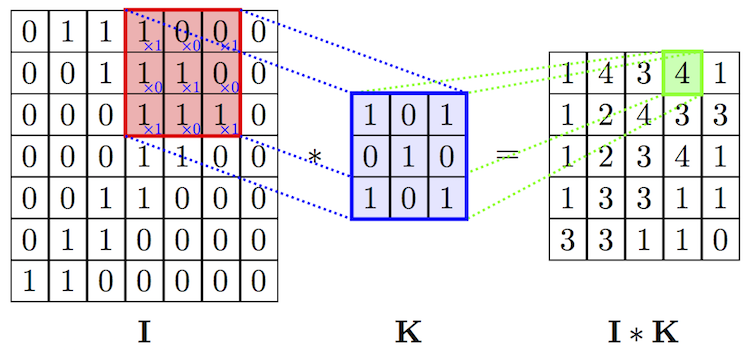
\includegraphics[scale=2]{convolution.png}
   \captionof{figure}{A kernel of size $1 \times 1 \times 3 \times 3$ convolving over activations of size $1 \times 1 \times 7 \times 7$, producing activations of size $1 \times 1 \times 4 \times 4$ in the next layer IMAGE CITATION SOURCE \cite{figconv}. } \label{figkonv}
\end{center}
\end{minipage}
\end{center}


The basic building block of the convolutional neural network is the convolution and the convolutional layer. It uses the learnable parameters $W^{(l)} \in \mathbb{R}^{C' \times C  \times k \times k}$, called a kernel, and is the before mentioned filter the network learns to apply to images. $C$ and $C'$ are the number of channels in layer $l$ and $l+1$ respectively. $k$ is a variable called the kernel size of the convolution \cite{cs231n}. 

The activations at layer $l+1$ are derived from the activations at layer $l$ by applying the kernel at every possible spatial location on the activations at layer $l$ (see figure \ref{figkonv}). Every neuron is multiplied by the value of the kernel at the same spatial location. The sum of all the products becomes the activation of a single neuron in layer $l+1$. Applying this operation on every region of neurons in the activation is called a convolution. The convolution operator is denoted by $*$ \cite{cs231n} \cite{convmath} \cite{convarithmetic}. 



A feature map in layer $l+1$ is the result of a single kernel of size $1 \times C  \times k\times k$ being convolved over the whole activation volume of the previous layer. $C'$ is the number of kernels a layer has and is also the number of feature maps the next layer will have \cite{cs231n} \cite{convmath}. 

The kernels have two additional non-learnable hyperparameters: a stride $s$ and zero-padding $p$. $s$ is the size of the step the kernel takes when it moves from one spatial location to the next during a convolution. The convolution in figure \ref{figkonv} has a stride of $s = 1$. Zero-padding entails padding the edges of the activation tensor with $p$ zeros (see figure \ref{figzeropad}). Since a convolution decreases the spatial size of the activations of the next layer, zero-padding is a way to control the size of the activations \cite{cs231n} \cite{convmath} \cite{convarithmetic}. 

\begin{center}
   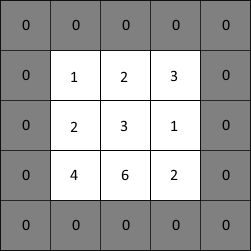
\includegraphics[scale=0.7]{zeropadding.png}
   \captionof{figure}{An activation with size $1 \times 3 \times 3$ is zero-padded with $p=1$ and the resulting tensor is of size $1 \times 5 \times 5$. White symbolizes the original tensor and grey symbolizes the padded zeros. }\label{figzeropad}
\end{center}
Miles, 17, of Niceville High School in 
Let $W^{(l)} \in \mathbb{R}^{C' \times C  \times k \times k}$, $X^{(l)} \in \mathbb{R}^{R \times C  \times (H+2p) \times (W+2p)}$ and $X^{(l+1)} \in \mathbb{R}^{R \times C'  \times H' \times W'}$. The dimensions of layer $l+1$ are defiend by equations \eqref{eqkonvW} and \eqref{eqkonvH} \cite{cs231n} \cite{convmath} \cite{convarithmetic}: 
\begin{equation}\label{eqkonvW}
W' = \frac{W-k+2p}{s} +1
\end{equation}
\begin{equation}\label{eqkonvH}
H' = \frac{H-k+2p}{s} +1
\end{equation}
The following equation defines the convolutional layer algebraically \cite{cs231n} \cite{convmath}:
\begin{equation}\label{konvolution}
\begin{split}
	\begin{bmatrix} X^{(l+1)} \end{bmatrix}_{r, c', h', w'}	
		& = X^{(l)}_{r, c', h', w'} *W^{(l)}_{c'} \\
		& = \sum^{C-1 }_{c=0} \sum^{k-1 }_{j=0} \sum^{k-1 }_{i=0} X^{(l)}_{r, c, (1+sh'-s+j), (1+sw'-s+i)}W^{(l)}_{c', c, j, i}
\end{split}
\end{equation}

The index of the term which shall be used to convolve specifies which dimensions will be convolved upon and summed over. For instance, $W^{(l)}_{c'}$ implies that the $C$, $H$ and $W$ dimensions (all channels) should be used in the convolution, while $W^{(l)}_{c', c}$ implies that only the $H$ and $W$ dimension (one channel) should undergo the convolution operation.

Convolutions are in practice implemented with the functions $row2im$ and $im2row$ which enable the convolution to be computed with a single dot product \cite{cs231n} \cite{convmath} \cite{convarithmetic}. The underlying math is equivalent with the equations shown in this paper. However, $row2im$ and $im2row$ are outside of the scope of this paper and are left to the reader to research if a more computationally efficient implementation is required. 

\subsubsection{Backpropagation}
At every layer $l$ the delta-error of the proceeding layer $\delta^{(l+1)}$ has to be backpropagated to create the delta-error at the current layer. $\delta^{(l)}$ is then used to compute the partial derivatives of the loss with respect to the weights $W^{(l)}$ to be used in the gradient \cite{cs231n} \cite{convmath}. 
 
The backpropagation of the recursive delta-error $\delta^{(l+1)}$ is derived by the use of the chain rule. $\delta^{(l+1)} = \inpd{L(\theta)}{X^{(l+1)}}$ is broken up into two smaller partial derivatives $\inpd{L(\theta)}{X^{(l+1)}}$ and $\inpd{X^{(l+1)}}{X^{(l)}}$. Additionally, because more than one single neuron in layer $l$ is responsible for the delta-error at layer $l+1$, all the neurons of layer $l$ have to be summed over, similar to equation \eqref{dLdX_FCC}, \eqref{dLdW_FCC}, and \eqref{dLdb_FCC}. This can be done since the derivative of a sum is equivalent to the sum of the derivatives of each element. $X^{(l+1)}_{r,c',h',w'}$ is then replaced by its definition from equation \eqref{konvolution} \cite{convmath} \cite{webconv1} \cite{webconv2} \cite{webconv3}: 

\begin{equation}\label{konvolutionbackprop}
\begin{split}
	\delta^{(l)}_{r,c,h,w}
		& = \pd{L(\theta)}{X^{(l)}_{r,c,h,w}} \\
		& = \sum^{C' }_{c'=1} \sum^{H' }_{h'=1} \sum^{W' }_{w'=1} \pd{L(\theta)}{X^{(l+1)}_{r,c',h',w'}} \pd{X^{(l+1)}_{r,c',h',w'}}{X^{(l)}_{r,c,h,w}} \\
		& = \sum^{C' }_{c'=1} \sum^{H' }_{h'=1} \sum^{W' }_{w'=1} \delta^{(l+1)}_{r,c',h',w'} \pd{\sum^{C-1 }_{c=0} \sum^{k-1 }_{j=0} \sum^{k-1 }_{i=0} X^{(l)}_{r, c, (1+sh'-s+j), (1+sw'-s+i)}W^{(l+1)}_{c', c, j, i}}{X^{(l)}_{r,c,h,w}}
\end{split}
\end{equation}

Every partial derivative in the most inner sum will be equal to to zero if $X^{(l)}_{r, c, h'+j, w'+i} \neq X^{(l)}_{r,c,h,w}$. Using the substitutions $h = 1+sh'-s+j$ and $w = 1+sw'-s+i$ the three inner sums are cancelled out \cite{webconv1} \cite{webconv2} \cite{webconv3}:

\begin{equation}
\begin{split}
	\delta^{(l)}_{r,c,h,w}
		& = \sum^{C' }_{c'=1} \sum^{H' }_{h'=1} \sum^{W' }_{w'=1} \delta^{(l+1)}_{r,c',h',w'} \pd{\sum^{C-1 }_{c=0} \sum^{k-1 }_{j=0} \sum^{k-1 }_{i=0} X^{(l)}_{r, c, (1+sh'-s+j), (1+sw'-s+i)}W^{(l+1)}_{c', c, j, i}}{X^{(l)}_{r,c,h,w}} \\
		& = \sum^{C' }_{c'=1} \sum^{H' }_{h'=1} \sum^{W' }_{w'=1} \delta^{(l+1)}_{r,c',h',w'} W^{(l+1)}_{c', c, (h+s-1-sh'), (w+s-1-sw')}     \\
\end{split}
\end{equation}


Which one can see is a sum of convolutions (for the special case $s=1$) where a feature map of the delta-error of layer $l+1$ convolves over all the kernels of layer $l$ where the kernels are rotated by $180^\circ$. This is intuitive since every feature map in $X^{(l)}$ is used to create a single feature map in $X^{(l+1)}$.

The partial derivative of the loss $L(\theta)$ with respect to the weights $W^{(l)}$ is derived the same way the backpropagation of the error is derived. Now the $R$-dimension is additionally summed over since the loss is a function of every example in the mini-batch, and affects the gradient \cite{cs231n} \cite{webconv1} \cite{webconv2} \cite{webconv3}. 
\begin{align}
\begin{split}
	\pd{L(\theta)}{W^{(l)}_{c',c,h,w}}
		& = \sum^{R }_{r=1} \sum^{C' }_{c''=1} \sum^{H' }_{h'=1} \sum^{W' }_{w'=1} \pd{L(\theta)}{X^{(l+1)}_{r,c'',h',w'}} \pd{X^{(l+1)}_{r,c'',h',w'}}{W^{(l)}_{c',c,h,w}} \\
		& = \sum^{R }_{r=1} \sum_{c''=1}^{C' } \sum^{H' }_{h'=1} \sum^{W' }_{w'=1} \delta^{(l+1)}_{r,c'',h',w'} \pd{\sum\limits^{C-1 }_{c=0} \sum\limits^{k-1 }_{j=0} \sum\limits^{k-1}_{i=0} X^{(l)}_{r, c, (1+sh'-s+j), (1+sw'-s+i)}W^{(l)}_{c'', c, j, i}}{W^{(l)}_{c',c,h,w}} \\
		& = \sum^{R }_{r=1} \sum^{H' }_{h'=1} \sum^{W' }_{w'=1} X^{(l)}_{r, c, (1+sh'-s+h), (1+sw'-s+w)} \delta^{(l+1)}_{r,c',h',w'} \\
\end{split}
\end{align}

}

\headerbox{Dense Face Detection}{name=facedetection,span=1,column=2}{

\section{Dense Face Detection}

In this section we systematically and empirically investigate how to construct and improve a convolutional-neural-network-based model to detect a variable number of faces in an image. Every factor and suggestion which affects the model performance is evaluated one by one and added to a baseline model, which we name FaceNet.

\subsection{Background}
\subsubsection{WIDERFace}
For the task of detecting a variable number of faces in an iamge, the WIDERFace dataset \cite{WIDERFace} was used. It is a dataset consisting of 32 203 images of a total of 393 703 number of faces at different scales, lighting and occlusions. Every training example consists of a number of bounding boxes which describes all the faces in the image. A bounding box consists of four coordinates specifying its location: two for the upper left corner and two for the bottom right corner of the bounding box. The images are labeled by humans and is called the ground truth of the image.

\subsubsection{One-shot detectors}
One-shot detectors were first introduced by the model YOLO \cite{yolo} and later modified and improved by the models SSD \cite{ssd}, YOLO9000 \cite{yolo9000}, DSSD \cite{dssd} and RetinaNet \cite{retinanet}. A one-shot detector works by predicting up to tens of thousands of bounding boxes in different spatial positions in an image, that sets out to detect every object in that image. For every set of predetermined spatial positions in the image, the model predicts 4 bounding box coordinates and probability scores that there exists an object inside the specified bounding box.

The model is trained by assigning every bounding box either a negative or a positive label during training, depending on if the bounding box contains a ground truth object or not. A bounding box is said to contain an object if the intersection over union (IoU) \cite{iou} of the area of the bounding box and the area of the ground truth is bigger or equal to a threshold value (0.55). The intersection over union is used to determine how similar two sets $A$ and $B$ are (see figure \ref{figiou}). It is bounded by the interval $[0,1]$ and is defined by the following equation: 

\begin{equation}\label{eqiou}
IoU(A, B)=\frac{|A \cap B|}{|A \cup B|}
\end{equation}


\begin{center}
   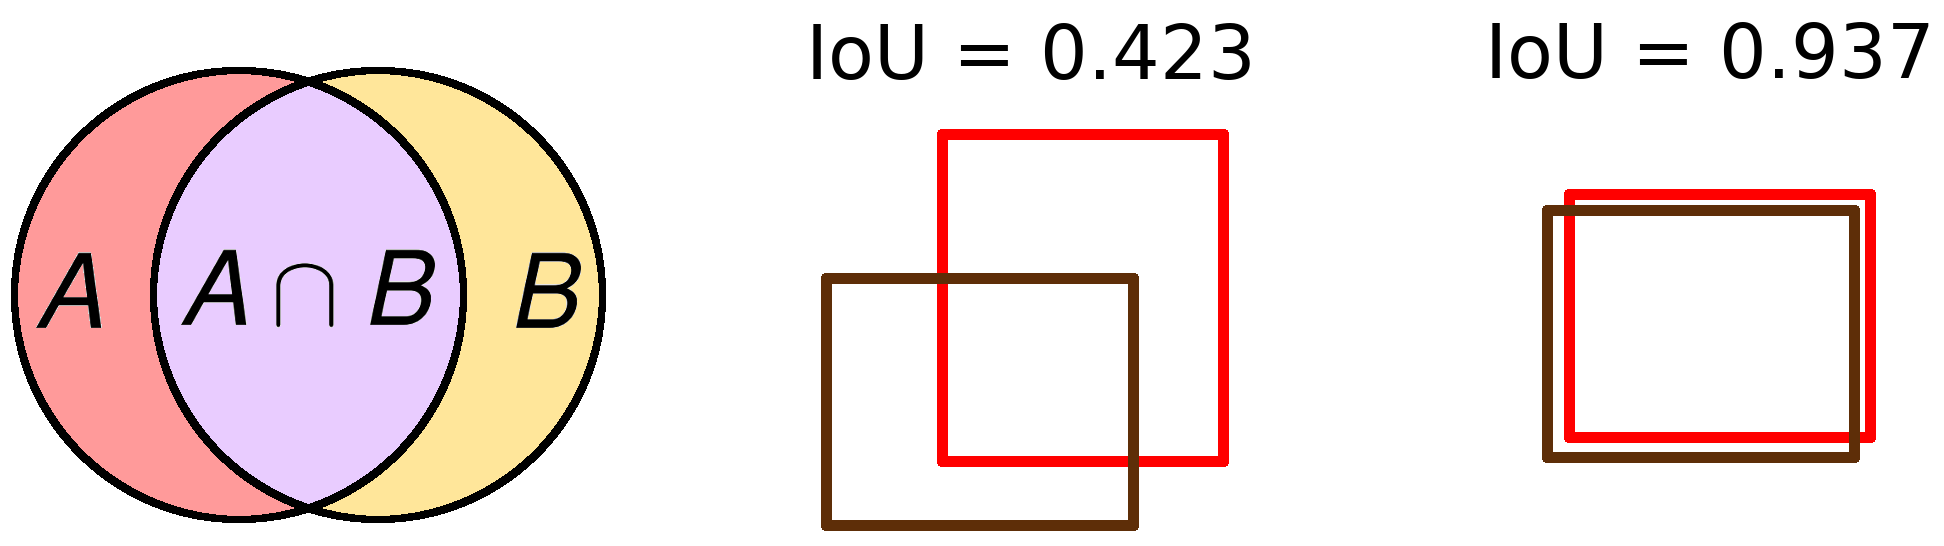
\includegraphics[scale=0.7]{iou.png}
   \captionof{figure}{IoU \cite{iou} is defined as the size of the union divided by the size of the intersection of two sets $A$ and $B$. A bigger IoU implies that the predicted bounding box is closer to the ground truth. } \label{figiou}
\end{center}

\subsection{Method}
\subsubsection{FaceNet Baseline Model}
The baseline model uses the deep residual convolutional neural network ResNet-18 \cite{resnet} as a backbone network and feature extractor. It uses a total of 18 convolutional layers throughout blocks named \textit{conv1} to \textit{conv5} to extract features from the input image. An additional \textit{conv6} block is created after the last layer to create one additional scale of feature maps. The block consists of one convolutional layer with stride 2, and 2 residual bottleneck layers used by Resnet-50 up to ResNet-152. The feature maps created by the backbone model is then fed into two smaller sub-networks, called the classification head and the regression head. They are constructed out of 4 residual bottleneck layers.

Bounding boxes are created from a number of anchor boxes at every spatial position (width and height) from a set of feature maps. An anchor box is a bounding box of a specific size and scale, used to base the bounding box predictions off. Anchor boxes used by FaceNet are set to be of sizes in the range $[16, 406]$ pixels, each increasing by a factor of $2^{1/3}$ for every new anchor box size. Two ratios of width:height are used at every scale, namely $1:\frac{2}{3}$ and $1:1$, to enable the detection of faces facing sideways and directly into the camera. Having densely packed anchors makes it that every ground truth bounding box (of sufficient size) has an IoU$>0.55$ with at least one anchor box. The anchor boxes are spaced out to include 3 scales with 2 aspect ratios across feature maps from the levels \textit{conv2} to \textit{conv5}, to enable the detection of faces of different scales, similar to RetinaNet \cite{retinanet}.

The regression and classification sub-networks take in the last convolutional output from a single network level (\textit{conv2} to \textit{conv5}) as input. Let $W$ and $H$ be the width and height of the tensor of activations at a single network level, and $C$ be the amount of classes to classify. FaceNet uses $C=2$, one for a background class (no face) and one for a foreground class (a face). The classification head predicts $C$ probabilities for every anchor $A$, that there exists a face in the anchor box at every spatial location ($W \times H$), for a total of $KWHA$ values. The regression head predicts $4$ coordinate offsets for every point of the anchor box, for it to match the ground truth as closely as possible, for a total of $4WHA$ coordinate offsets. Additionally, similar to RetinaNet \cite{retinanet}, the last conventional layer which predicts class probabilities uses a bias $b = -\log{\frac{C(1-\pi)}{\pi}}$, such that the model, when first initialized, predicts a probability of $\pi$ for the case of there existing a foreground class (a face) in every bounding box. The value $\pi = 0.001$ was used.

\subsubsection{Training}
If not otherwise stated, each version of FaceNet was trained for 70 000 iterations on an Nvidia GTX 1080ti with an initial learning rate of 0.0001, and lowering the learning rate by a factor of 10 after 50 000 and 60 000 iterations. Due to memory limitations a batch size of 8 is used. The models are trained on square image crops, randomly picked to be of between 0.33 and 0.95 of the short size of the image, and resized to be of size $512^2$ pixels. This is done to artificially increase the size of the training data. Additionally, the image is flipped horizontally with a probability of 0.5.

The models are evaluated on the WIDERFace validation set, using the easy, medium and hard splits provided by the WIDERFace evaluation server. The evaluation metric used is mean average precision (mAP). It is calculated by plotting the accuracy of the model as a function of its recall. The mean average precision is given by the integral of the accuracy with respect to the recall. The models will be evaluted on the easy, medium and hard validation splits.

\subsection{Experiments}
In the following sections we systematically change and evaluate one network architecture decision at a time, to iteratively improve the FaceNet model. Since we test 8 different factors, a total of 128 different models need to be trained to thoroughly test every single combination of factors, something which we cannot do due to limited computational resources. Thus, we employ our iterative method of improving the FaceNet model one factor at a time.

\subsubsection{Baseline}
The loss function for the FaceNet baseline (FaceNet v1.0) is constructed out of the sum of a coordinate regression loss $L_r$, and a bounding box classification loss $L_c$. The basline model uses $L_r$ which is the Smooth L1 Loss \cite{cs231n} defined by equation \eqref{eqsmoothl1loss}, and $L_c$ which is softmax cross entropy across two classes, the foreground class for the case that a face does exist and does not exist respectively inside a given anchor box.

The total loss $L(\theta)$ is the mean of the regression losses $L_r$ of all positively assigned anchors plus the mean of the classification losses of all anchors. Negatively assigned anchors do not have any effect on the regression loss. Let $r_a$ and $\hat{r}_a$ be the predicted and ground truth coordinate offsets for anchor box $a$. Let $p_a$ and $\hat{p}_a$ be the predicted and ground truth probability score respectively, for anchor $a$ to contain a face. Let $N$ be the set containing all anchor boxes $a$, and $N_{pos}$ be the set containing every positively assigned anchor box. The total loss is defined as:

\begin{equation}\label{eqfacenetsoftmax}
L_r(x) = \begin{cases}
				0.5x^2 & \mbox{if } |x| < 1\\
				|x| - 0.5 & \mbox{otherwise}\\
			\end{cases}
\end{equation}
\begin{equation}\label{eqsmoothl1loss}
L_c(p, \hat{p}) = -p \log{\hat{p}}
\end{equation}
\begin{equation}
\begin{split}
	L(\theta) = &  \frac{1}{|N|} \sum_{a \in N} L_c(p_a, \hat{p}_a) 
	 + \frac{1}{|N_{pos}|} \sum_{a \in N_{pos}} L_r(r_a - \hat{r}_a)  \\ 
\end{split}
\end{equation}

When evaluated on the WIDERFace validation set, the model achieved an mAP of 0 across all 3 sets: easy, medium and hard. The model converged to classify every single bounding box as a negative example, resulting in no faces being found in any image.

\subsubsection{Loss Functions}
One observed problem with the baseline was an unstable loss function. The loss function varied between values of 0 and 8000 for any arbitrary training example. We dealt with this problem by following the work of SSD \cite{ssd} and RetinaNet \cite{retinanet}, and normalizing the classification loss by the total number of positively assigned bounding boxes, $|N_{pos}|$, instead of the total number of bounding boxes $|N|$.

Additionally, the baseline model uses a softmax function to draw its classification prediction from, based on two values; one for each object class. An open source implementation of YOLO \cite{sigmoidvssoftmax} showed that using a binary cross entropy loss function (logistic regression), instead of a categorical cross entropy using a softmax function, led to a gain in mAP. For FaceNet v1.1, the softmax layer in FaceNet is replaced by the sigmoid function, and binary cross entropy is used instead. Let the new classification loss and total loss be denoted by $L_c$ and $L(\theta)$ respectively. The total loss is defined by the following equations:

\begin{equation}
L_c(p, \hat{p}) = -p \log{(\hat{p})} -(1-p) \log{(1-\hat{p})}
\end{equation}

\begin{equation}
\begin{split}
	L(\theta) = &  \frac{1}{|N_{pos}|} \sum_{a \in N} L_c(p_a, \hat{p}_a) 
	 + \frac{1}{|N_{pos}|} \sum_{a \in N_{pos}} L_r(r_a - \hat{r}_a)  \\ 
\end{split}
\end{equation}

Focal loss, used by RetinaNet \cite{retinanet}, introduced a loss function that focused on the training examples which were hard to classify. It was shown that using focal loss instead of cross entropy for multi-class object detection increased the final accuracy of the model. Let $L_f$ denote the focal loss, which is used as the classification loss by FaceNet v1.2:

\begin{equation}
L_f(p, \hat{p}) = -p (1-p)^\gamma \log{(\hat{p})} -(1-p) p^\gamma\log{(1-\hat{p})}
\end{equation}

Since FaceNet proposes more bounding boxes compared to RetinaNet, a $\gamma$ value of 3 was used, instead 2 used by RetinaNet, to offset the increase in bounding boxes. Focal loss is robust to the changes in $\gamma$, and thus the chosen value should not have a considerable effect on the accuracy.

When evaluated on the easy/medium/hard splits of the WIDERFace validation set, FaceNet v1.1 achieved an mAP of 37.4/21.7/9.7, while FaceNet v1.2 achieved an mAP of 22.4/12.1/5.1. The model using focal loss performed considerably worse; an average decrease of 10 points in mAP.

\subsubsection{Feature Pyramid Network}
Using a feature pyramid network (FPN) together with a standard backbone ResNet network has been shown to yield higher detection and classification accuracies \cite{fpn} \cite{retinanet} for multi-class object detection. Instead of only basing the face predictions of the feature maps from $conv2$ to $conv6$ of the backbone network, a top-down architecture from the FPN is used to enable the feature maps at lower scales to make use of higher level features. FaceNet v1.3 uses the previously best performing binary cross entropy as its classification loss, while FaceNet v1.4 uses the focal loss.

Adding an FPN to FaceNet yielded a dramatical increase in mAP: The model's results on the easy/medium/hard splits for version 1.3 were 89.3/85.9/65.9, a 1200\% increase in mAP on the hard set. The version incorporating focal loss, FaceNet v1.4, performed slightly worse, achieving an mAP of 81.0/81.0/64.2.

The loss function was modified once again to study the effects it had on the accuracy: Instead of normalizing all the losses by the total number of positively assigned anchors, each classification and regression loss is computed separately at every pyramid level. Let $P$ be the set of all pyramid levels $p$, $N^p$ be the set of all created anchor boxes at every spatial position at pyramid level $p$, and $N^p_{pos}$ be the set of all positively assigned anchors at pyramid level $p$. The new total loss $L(\theta)$ is defined by:

\begin{equation}
\begin{split}
	L(\theta) = & \sum_{p \in P} \frac{1}{|N^p_{pos}|} \sum_{a \in N^p} L_c(p_a, \hat{p}_a) \\
	 & + \sum_{p \in P}  \frac{1}{|N^p_{pos}|} \sum_{a \in N^p_{pos}} L_r(r_a - \hat{r}_a)  \\ 
\end{split}
\end{equation}

FaceNet versions 1.5 and 1.6 used the new level-separated loss with binary cross entropy and focal loss respectively as their classification loss. These versions performed slightly worse than the previous non-level-specific versions. The results on the easy/medium/hard set were 87.2/82.5/50.4 mAP for the model using binary cross entropy and 85.1/80.0/50.6 mAP for the model using focal loss.

\subsubsection{Online Hard Example Mining}
Online hard example mining (OHEM) \cite{ohem} has been shown to increase mAP when training region based object detectors. Models using OHEM only train on the top $k$ bounding box classification errors, after non-maxima supression (NMS) is applied, in an effort to balance the ratio of negative to positive bounding boxes. Since FaceNet predicts approximately 250 000 bounding boxes for an image of size $512^2$ pixels, the ratio of negatively to positively assigned bounding boxes is high. FaceNet v1.7 uses OHEM separetely on every image in the mini-batch, and picks out the top 128 classification losses to backpropagate, after NMS is applied, to avoid duplicate regions.

Using OHEM resulted in a decrease in performance, halving the accuracy on the easy set, compared to the previously best performing model FaceNet v1.3. Quantitative results showed that the model had difficulties detecting large faces. When evaluated on the easy/medium/hard splits, v1.7 achieves an mAP of 46.0/51.8/42.3.

Applying the OHEM algorithm on the whole mini-batch, instead of applying it on every image separately, yielded faster training times and higher accuracies. A top $k$ value of 128 was used. The results on the easy/medium/hard set were 55.9/36.8/15.6 mAP. This version of OHEM performed worse than the previous image-specific version.

\subsubsection{New Features}
For FaceNet v1.9, a new anchor width to height ratio was used, namely 1:1.5. Looking at quantitative results of anchor assignment showed that the 1:2 width to height ratio resulted in anchor boxes which were always bigger than the ground truth in the training images. Adjusting the ratio accordingly should in theory lead to better quality final bounding boxes requiring less precise coordinate offsets, and a higher number of assigned ground truth bounding boxes. To offset the higher number of assigned bounding boxes, a higher IoU threshold was used: 0.65.

Empirical results on the easy/medium/hard shows that the model attained an mAP of 88.7/86.4/ 64.8. The model performed marginally worse than its earlier, lower threshold version.

Instead of using features from block \textit{conv2}, which is very computationally expensive, FaceNet v2.0 uses features starting from \textit{conv3}, in an effort to increase its efficiency and speed. Using features from a deeper layer may also enable the model to give more accurate predictions as an effect of a deeper architecture. A \textit{conv7} layer is added, similarly to the \textit{conv6} layer, to offset the increase in depth to still be able to predict bounding boxes of size $16^2$ to $416^2$ pixels. All other model details are the same as in v1.9.

FaceNet v2.0 achieves an mAP of 84.4/83.4/57.1 on the easy/medium/hard validation splits. Continuously sliding a face across a video feed, which was used as the input to the model, showed that the model fails to predict faces at regularly spaced out areas in the image. This shows that the current anchor boxes are too spaced out across the image, leading to ground truths sometimes not being assigned to an anchor during training.

To fix the problems of version 2.1, bi-linear interpolation is added to the classification and regression head. After the first 2 residual bottleneck layer, the feature maps were upscaled by a factor of 2. This will in turn create more spaced out anchor boxes across the final image. Results on the easy/medium/hard validation splits were 89.1/86.6/64.4

FaceNet v2.2 evaluated the previously best performing anchor box threshold value of 0.55, using the model architecture of FaceNet v2.1. Changing the threshold to the previously best performing threshold decreases the performance of the model. Results on the easy/medium/hard validation splits were 87.1/84.1/61.3 mAP.

Augmenting the training data with random color jitter, through adding random noise and shifting the hues by a random value, was shown in our experiments to increase accuracy. The model using color jitter is FaceNet v2.3. Results on the easy/medium/hard validation splits were 89.5/87.7/67.4 mAP, when all other factors remained constant from the previous FaceNet version.

Even though the model performs better with using features from \textit{conv2} to \textit{conv6}, a change to \textit{conv3} to \textit{conv7} has to be done for the following reason: The model performs badly on the hard WIDERFace split, which consists of many small faces. This is due to there not being any anchor boxes of sufficient size for any small ground truth to get assigned to an anchor, thus resulting in the model not learning to detect small faces. To deal with this issue, three additional anchor scales, $\{8^2, 10^2, 13^2\}$, are added, for a final scale coverage of $8^2$ to $416^2$ pixels. Feature maps used by FaceNet v2.4 are \textit{conv2} to \textit{conv7}, to have a sufficiently dense anchors to guarantee the ground truth has a minimum IoU overlap of 0.65 with at least one anchor box. Using features from \textit{conv1} is too computationally inefficient and will use up too much vRAM, which our GPU has limited availability of. Therefore, the transition to \textit{conv2} to \textit{conv7} features has to be done.

This change led to an increase in mAP on the hard set, with a minimal decrease in mAP on the easy and medium sets: Results on the easy/medium/hard validation splits were 88.5/85.6/72.3 mAP.

\subsubsection{Increased Depth}
Since an increase in network depth increases training times and model size, and thus being limited by the GPU memory, this factor was tested last. FaceNet 2.5 uses the architecture of the best performing model so far, version 2.4, only varying the network depth. Experimentation showed that the network failed to converge using ResNet-50, ResNet-101 and ResNet-152 as backbone networks. The models resulted to predict only negative bounding boxes at every location in the image, similar to the baseline FaceNet v1.0. Due to the increase in memory, the batch size had to be lowered. This might have been a factor in the failure of effective convergence. An mAP of 0 was reached for all models with increased depth.

\subsubsection{Final Model Results}
The experiments are summarized in table \ref{tablefacenet}. The best performing models FaceNet v2.4 for the hard split, and FaceNet v2.3 for the easy and medium splits, complete one forward iteration in 24ms and 22ms respectively. This enables the model to run approximately 50 times a second. Quantitative results on the WIDERFace validation set can be seen in figure \ref{figwiderfaceval}

\begin{minipage}{\linewidth}
   \centering
   \captionof{table}{\textbf{FaceNet Face Detection}. A table comparing the different FaceNet versions.}
   \label{tablefacenet}
   \begin{tabular}{| c | c | c | c | c | c | c | l | l | l |}
    \hline
    Model & Features & BCE & FL & FPN & OHEM & Jitter & mAP$_{e}$ & mAP$_{m}$ & mAP$_{h}$\\  \hline
    v1.0 & \textit{conv2}-\textit{conv6} &  &  &  & && 0& 0&0 \\ \hline 
    v1.1 & \textit{conv2}-\textit{conv6} &  \ding{52} &  &  & && 37.4& 21.7& 9.7 \\ \hline 
    v1.2 & \textit{conv2}-\textit{conv6} &  & \ding{52} &  & && 22.4& 12.1& 5.1\\ \hline 
    v1.3 & \textit{conv2}-\textit{conv6} &  \ding{52}&  & \ding{52} && & 89.3 & 85.9 & 65.9 \\ \hline 
    v1.4 & \textit{conv2}-\textit{conv6} &  & \ding{52} & \ding{52} & && 81.0& 81.0&  64.2\\ \hline 
    v1.7 & \textit{conv2}-\textit{conv6} & \ding{52} &  & \ding{52} & \ding{52} && 46.0 & 51.8 &42.3 \\ \hline 
    v1.8 & \textit{conv2}-\textit{conv6} & \ding{52} &  & \ding{52} & \ding{52} && 55.9& 36.8& 15.6\\ \hline 
    v2.0 & \textit{conv3}-\textit{conv7} & \ding{52} &  & \ding{52} & && 84.4& 83.4& 57.1\\ \hline 
	v2.1 & \textit{conv3}-\textit{conv7} & \ding{52} &  & \ding{52} & && 89.1& 86.6& 64.4\\ \hline 
	v2.3 & \textit{conv3}-\textit{conv7} & \ding{52} &  & \ding{52} & & \ding{52}& \textbf{89.5}& \textbf{87.7}& 67.4\\ \hline
	v2.4 & \textit{conv2}-\textit{conv7} & \ding{52} &  & \ding{52} & & \ding{52}& 88.5& 85.6& \textbf{72.3}\\ \hline 
    \end{tabular}
\end{minipage}


\begin{center}
   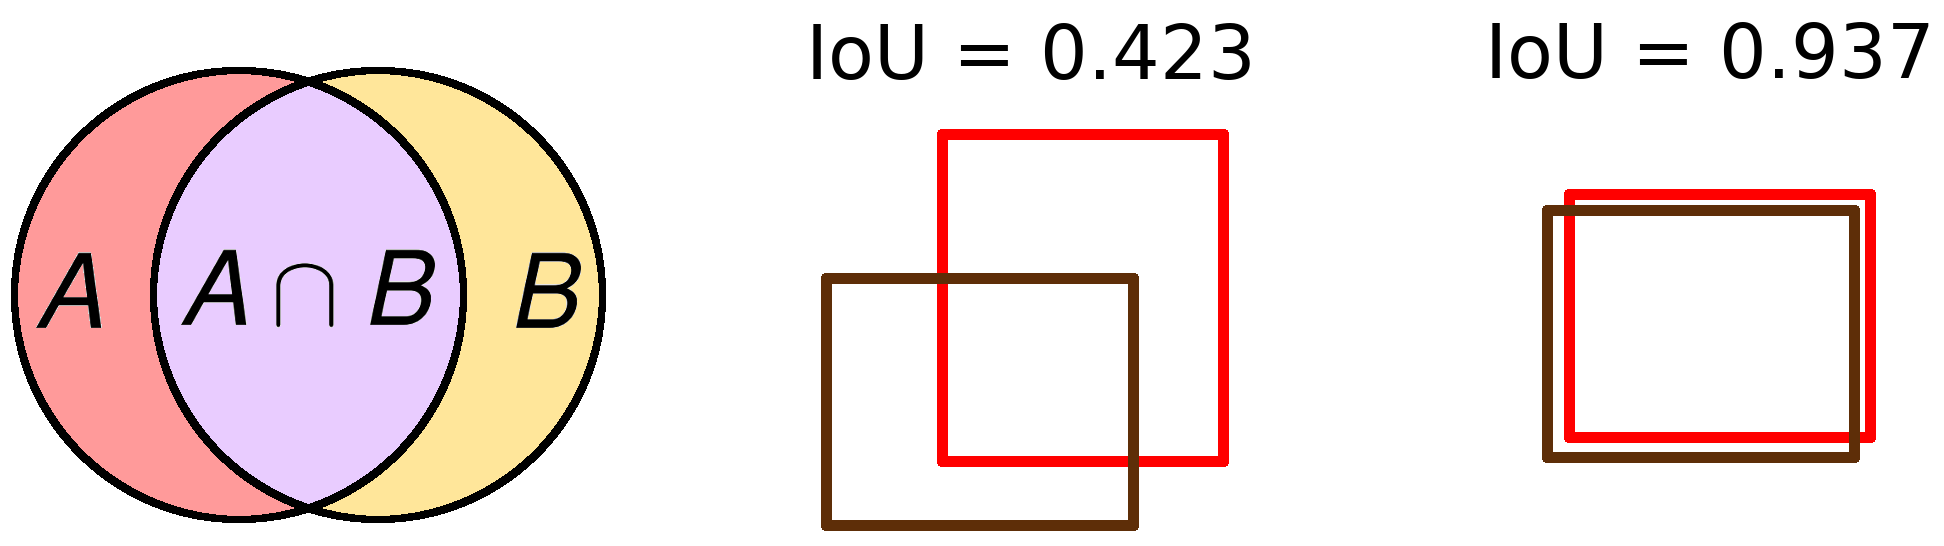
\includegraphics[scale=0.7]{iou.png}
   \captionof{figure}{figfacedetection.png}\caption{The detections of FaceNet v2.3 on four images of the WIDERFace validation set \cite{WIDERFace}.} \label{figwiderfaceval}
\end{center}

\subsection{Discussion}
Contrary to research done on multi-class object detection, various methods which have shown to increase accuracy, such as online hard example mining and focal loss, has led to a decrease in accuracy. Using networks of larger depth, as research \cite{retinanet} \cite{resnet} shows, should also increase the accuracy of models, but the present study reached the opposite conclusion.

One reason for which the deeper networks, ResNet-50, ResNet-101 and ResNet-151, failed to detect any positive examples, might be the batch size. Since the early experiments used a ResNet-18 as a backbone network, a larger batch size could be used due to smaller model size. This larger batch size could reduce the stochasticity of SGD by giving a more accurate approximation of the true gradient. Using a small batch size could have led the model to converge to only detect negative bounding box suggestions.

The final model is capable of running in faster than real time speeds, approximately 50 times a second, for an image of size $512^2$ pixels. It is sufficiently accurate and computationally efficient to be used for real time video, to serve as a baseline model for any system incorporating surveillance, security or detection of humans.


}

%%%%%%%%%%%%%%%%%%%%%%%%%%%%%%%%%%%%%%%%%%%%%%%%%%%%%%%
%%%%%%%%%%%%%%%%%%%%%%%%%%%%%%%%%%%%%%%%%%%%%%%%%%%%%%%
%%%%%%%%%%%%%%%%%%%%%%%%%%%%%%%%%%%%%%%%%%%%%%%%%%%%%%%
%%%%%%%%%%%%%%%%%%%%%%%%%%TCN%%%%%%%%%%%%%%%%%%%%%%%%%%
%%%%%%%%%%%%%%%%%%%%%%%%%%%%%%%%%%%%%%%%%%%%%%%%%%%%%%%
%%%%%%%%%%%%%%%%%%%%%%%%%%%%%%%%%%%%%%%%%%%%%%%%%%%%%%%
%%%%%%%%%%%%%%%%%%%%%%%%%%%%%%%%%%%%%%%%%%%%%%%%%%%%%%%

\headerbox{Improving TCNs for Image Captioning}{name=tcn,span=1,column=3}{

\section{Improving TCNs for Image Captioning}
}

\headerbox{Background}{name=background,span=1,column=3, below=tcn}{
In conventional convolutional neural networks, the model learns to transform a given input by learning to apply a number of two-dimensional discrete convolutions on the input data. Instead of convolving along the spatial dimensions, a convolutional neural network can be used to convolve along the time dimension, and can thus be used as a sequence model for time series data, as long as there is no information leakage from the future into the past. Recent work on Temporal Convolutional Networks (TCN) \cite{tcn} shows that the convolutional model outperforms its recurrent neural network (RNN) variants, including Long Short Term Memory (LSTM), and Gated Recurrent Units (GRU), on a variety of tasks. 
\vspace{11pt}

I suggest the following two improvements regarding zero-padding and dilation:
}

\headerbox{Background}{name=background,span=1,column=3, below=tcn}{
In conventional convolutional neural networks, the model learns to transform a given input by learning to apply a number of two-dimensional discrete convolutions on the input data. Instead of convolving along the spatial dimensions, a convolutional neural network can be used to convolve along the time dimension, and can thus be used as a sequence model for time series data, as long as there is no information leakage from the future into the past. Recent work on Temporal Convolutional Networks (TCN) \cite{tcn} shows that the convolutional model outperforms its recurrent neural network (RNN) variants, including Long Short Term Memory (LSTM), and Gated Recurrent Units (GRU), on a variety of tasks. 
\vspace{11pt}

I suggest the following two improvements regarding zero-padding and dilation:
}

\headerbox{Background}{name=background,span=1,column=3, below=tcn}{
In conventional convolutional neural networks, the model learns to transform a given input by learning to apply a number of two-dimensional discrete convolutions on the input data. Instead of convolving along the spatial dimensions, a convolutional neural network can be used to convolve along the time dimension, and can thus be used as a sequence model for time series data, as long as there is no information leakage from the future into the past. Recent work on Temporal Convolutional Networks (TCN) \cite{tcn} shows that the convolutional model outperforms its recurrent neural network (RNN) variants, including Long Short Term Memory (LSTM), and Gated Recurrent Units (GRU), on a variety of tasks. 
\vspace{11pt}

I suggest the following two improvements regarding zero-padding and dilation:
}





\headerbox{7. References}{name=references,column=0,span=1,below=p3,above=bottom}{



%\small % Reduce the font size in this block
\renewcommand{\section}[2]{\vskip 0.05em} % Get rid of the default "References" section title
%\nocite{*} % Insert publications even if they are not cited in the poster


\bibliographystyle{unsrt}
\bibliography{poster} % Use sample.bib as the bibliography file
}

\end{poster}

\end{document}
